\section{Ход работы, результаты}

\subsection{Описание установки}
В нашем случае установка оборудована <<горизонтальной щелью>>. Ее схема представлена на рис. \ref{fig:schema1}. Свет от источника Л проходит через красный монохроматический фильтр, фокусируется колиматором К на щели S. После этого пучек становится параллельным, проходя линзу $O_1$. дифракцияагируя в кювете, он вновь попадает на собирающую линзу $O_2$, фокусируясь в плоскости наблюдения микроскопа.

В кювету погружен генератор УЗ волн, глубина погружения регулируется микрометрическим винтом, частота~--- генератором переменного тока и частотомером. Изменяя частоту, установлена четкая дифракцияакционная картина в поскости винта, что соответствует генерации стоячей волны в кювете. дифракцияакционные полосы ориентированы горизонтально.
Растояние между ними измеряется микрометрическим винтом В.

\begin{figure}[!h]
	\centering
	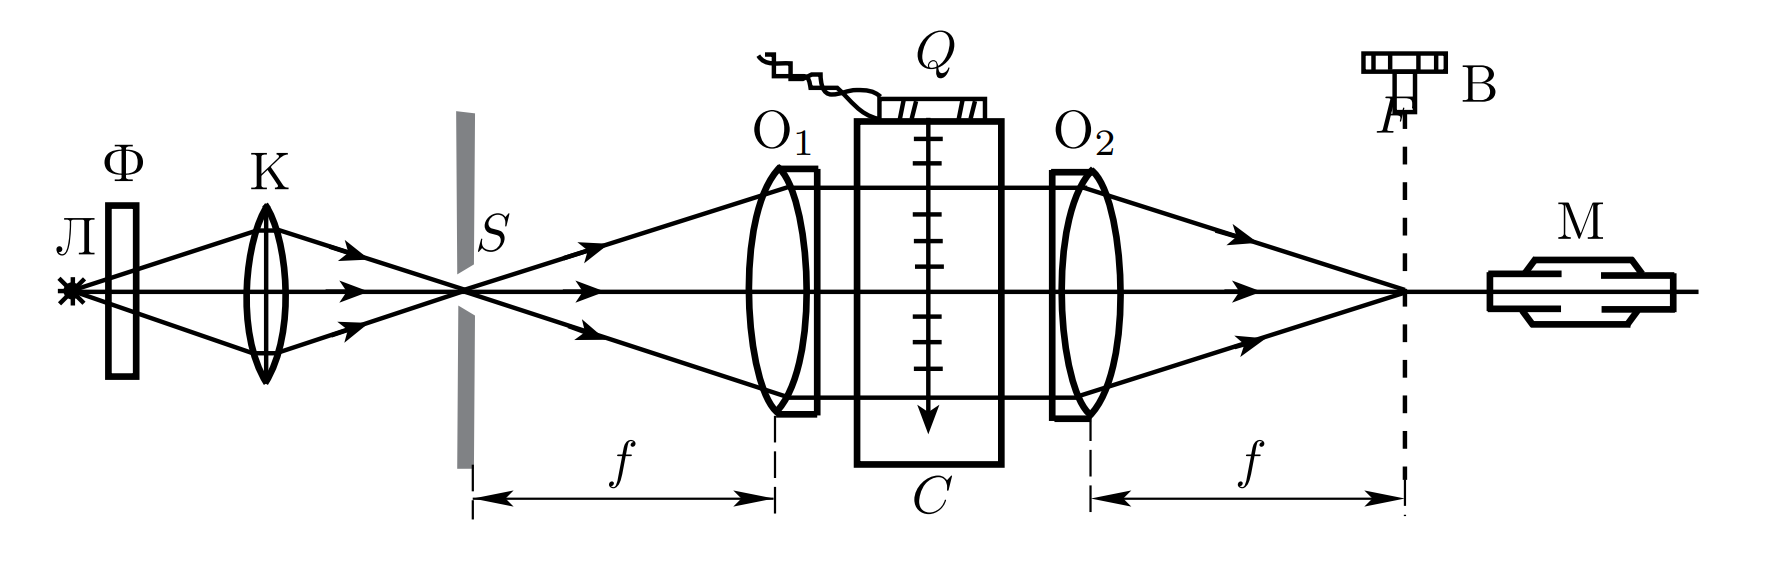
\includegraphics[width=0.6\linewidth]{pics/schema1.png}
	\caption{Схема установки для наблюдения дифракции на акустической фазовой                   решетке.}
	\label{fig:schema1}
\end{figure}

\subsection{Оценка скорости ультразвука по дифракционной картине}
Оценить длину УЗ-волны в воде можно как удвоенное расстояние между соседними положениями УЗ-излучателя, соответствующими наиболее чёткими дифракционными картинами. 
Полченные предварительно оценочные значения: 
\begin{gather*}
    x_1 = (1370 \pm 5) \text{мкм}, \\
    x_2 = (242 \pm 5) \text{мкм}, \\
    \lambda \approx 2 \cdot (x_2 - x_1) = (2260 \pm 10) \text{мкм}.
\end{gather*}
Рабочая частота генератора в оценочном опыте: $\nu = (1,132 \pm 0,001)$ МГц. Таким образом, оценка скорости звука:
\[
v \approx \Lambda \cdot \nu = (2490 \pm 40) \text{м/с}.
\]
Полученное значение сходится по порядку с табличным значением в приблизительно $1500$ м/c.

\subsection{Определение скорости ультразвука по дифракционной картине}
Используя соотношение \ref{eq:1}, по координатам дифракцияакционных полос определим скорость УЗ-волн в воде. Положение полос определены при помощи микрометрического винта. Длина волны красного света: $\lambda = (640 \pm 20)$нм. Фокусное расстояние линзы: $F = 30$см. Результаты измерений и расчетов представлены в таблице и графике 1.

\begin{table}[!ht]
    \centering % ахахахах, тогда да
    \begin{tabular}{|l|l|l|l|l|l|l|l|l|l|}
    \hline
        $\nu, $МГц & $x_{-3}$ & $x_{-2}$ & $x_{-1}$ & $x_0$ & $x_1$ & $x_2$ & $x_3$ & $l_1$ & $v$, м/с \\ \hline
        1,133 & -344 & -216 & -72 & 56 & 200 & 336 & 480 & 123 & 1651 \\ \hline
        0,988 & -308 & -176 & -64 & 56 & 184 & 308 & 428 & 122 & 1451 \\ \hline
        1,074 & -324 & -204 & -68 & 56 & 196 & 332 & 460 & 132 & 1458 \\ \hline
        1,163 & -372 & -220 & -76 & 56 & 204 & 348 & 496 & 144 & 1447 \\ \hline
        1,226 & — & -232 & -88 & 56 & 212 & 368 & — & 150 & 1465 \\ \hline
    \end{tabular}
\end{table}

Среднее значение скорости звука: $v = (1460 \pm 30) \text{м/с}$. Согласно справочным данным, при комнатной температуре скорость УЗ-волны в воде составляет около $1490 \text{м/c}$, отклонение полученного значения $\approx 2,3\%$.

\subsection{Определение скорости ультразвука методом тёмного поля}
Для данной части опыта между микроскопом и щелью установлена дополнительная линза $O$. При помощи калибровочной сетки была рассчитана цена деления окулярной шкалы микроскопа~--- 
$1 \text{дел} \sim \frac {1\text{мм}}{22}$.

Уменьшая частоту УЗ-волн, получена решетка, которую нельзя увидеть при открытом центральном максимуме, но видно, если закрыть последний проволочкой (см. метод темного поля). При этом полученная решетка не является сложной амплитудно-фазовой, так как возмущения жидкости малы и однородны.

При помощи окулряной шкалы микроскопа определены координаты первой и последней из хорошо видимых в поле зрения тёмных полос и число светлых промежутков между ними. Измерения проведены для нескольких частот, результаты в таблице. Расстояние между полосами соответствует половине длины волны.

\begin{table}[!ht]
\centering
\begin{tabular}{|l|l|l|l|l|l|l|}
\hline
$\nu$, МГц & $x_0$, дел & $x_1$, дел & $n$ & $l_1$, мм & $\Lambda$, мм & $v$, м/с \\ \hline
1.827 & 23 & 137 & 13 & 0.399 & 0.797 & 1456 \\ \hline
2.02 & 11 & 123 & 14 & 0.364 & 0.727 & 1469 \\ \hline
1.574 & 17 & 118 & 10 & 0.459 & 0.918 & 1445 \\ \hline
1.359 & 8 & 125 & 10 & 0.532 & 1.064 & 1445 \\ \hline
1.141 & 2 & 129 & 9 & 0.641 & 1.283 & 1464 \\ \hline
0.959 & 10 & 130 & 7 & 0.779 & 1.558 & 1495 \\ \hline
\end{tabular}
\end{table}

Среднее значение скорости~--- $v = (1460 \pm 23)\text{м/с}$. Отклонение от табличного значения составляет $\approx 1,9\%$.



%я тогда график сделаю для темного поля
%ты считай

% кк

%smb had a stroke B-)
%ого красивое
% и не говори)000


% Ты прикинь, оказывается, там 28см фокусное. Тогда получается еще лучше значение
%noice

\begin{figure}[h!]
\centering
\resizebox {0.75\textwidth} {!} {
\begin{tikzpicture} 
\begin{axis}[width=0.95\textwidth, height=\textwidth, xlabel = {$m$}, ylabel = {$Y$, мкм}, xmin = -3.5, xmax = 3.5, ymin = -400, ymax = 500, minor tick num = 5, legend style={legend style={at={(axis cs:-3.5, 500)},anchor=north west}}]
\addplot[color=black, mark=x, only marks] coordinates{
(-3, -344)
(-2, -216)
(-1, -72)
(0, 56)
(1, 200)
(2, 336)
(3, 480)
};
\addplot[color=blue, mark=o, only marks] coordinates{
(-3, -308)
(-2, -176)
(-1, -64)
(0, 56)
(1, 184)
(2, 308)
(3, 428)
};
\addplot[color=purple, mark=triangle, only marks] coordinates{
(-3, -324)
(-2, -204)
(-1, -68)
(0, 56)
(1, 196)
(2, 332)
(3, 460)
};
\addplot[color=red, mark=square, only marks] coordinates{
(-3, -372)
(-2, -220)
(-1, -76)
(0, 56)
(1, 204)
(2, 348)
(3, 496)
};
\addplot[color=black, mark=*, only marks] coordinates{
(-2, -232)
(-1, -88)
(0, 56)
(1, 212)
(2, 368)
};
\legend{$\nu = 1.133$ МГц, $\nu = 0.988$ МГц, $\nu = 1.074$ МГц, $\nu = 1.163$ МГц, $\nu = 1.226$ МГц}
\addplot[color=black, domain=-3:3]{134.4*x+62.9};
\addplot[color=blue, domain=-3:3]{122.3*x+61.1};
\addplot[color=purple, domain=-3:3]{131.7*x+64};
\addplot[color=red, domain=-3:3]{143.6*x+62.3};
\addplot[color=black, domain=-3:3]{150*x+63.2};
\end{axis}
\end{tikzpicture}
}
\caption{Графики зависимости координат $Y$ полос от их номера $m$ при разных частотах $\nu$}
\label{plot1}
\end{figure}

%%%%%%%%%%%%

\begin{figure}[h!]
\centering
\resizebox {0.5\textwidth} {!} {
\begin{tikzpicture}
\begin{axis}[xlabel = {$1/\nu$, МГц$^{-1}$}, ylabel = {$\Lambda$, мкм}, xmin = 0, xmax = 1.5, ymin = 0, ymax = 2, minor tick num = 5]
\addplot[color=black, mark=x, mark size=4, only marks] coordinates{
(0.55, 0.797)
(0.5, 0.727)
(0.64, 0.918)
(0.74, 1.064)
(0.88, 1.283)
(1.04, 1.558)
};
\addplot[color=blue, domain=0:1.5]{1.45*x};
\end{axis}
\end{tikzpicture}
}
\caption{График зависимости длины ультразвуковой волны $\Lambda$ от частоты $\nu$}
\label{plot2}
\end{figure}

\section{Выводы}
В работе установлено, что дифракционные методы на акустической фазовой решетке позволяют весьма точно определять параметры УЗ-волн, распространяющихся в воде. Метод тёмного поля оказался несколько более точным: в первом эксперименте отклонение от табличного значения составило 2,3\%, во втором~--- 1,9\%. Относительно небольшие значения погрешностей позволяют утверждать:
\begin{itemize}
    \item Использованные при выводе применённых формул приближения мало влияют на точность расчётов;
    \item На акустической решётке действительно наблюдается дифракция Фраунгофера;
    \item Акустическую решётку в данном эксперименте корректно считать чисто фазовой.
\end{itemize}